\documentclass[a4paper]{article}
\usepackage[14pt]{extsizes} 
\usepackage[utf8]{inputenc}
\usepackage[russian]{babel}
\usepackage{setspace,amsmath}
\usepackage{graphicx}
 \usepackage{mathtools}
\usepackage[left=10mm, top=15mm, right=15mm, bottom=15mm, nohead, footskip=10mm]{geometry} 
\begin{document}
\section{Задача 1}
Построить конечный автомат, распознающий язык:
\begin{enumerate}
  \item L = \begin{Bmatrix}
w \in \begin{Bmatrix}
a, b, c
\end{Bmatrix}* | |w|_{c} = 1
\end{Bmatrix}
\\ \includegraphics [scale=0.5]{2022-03-30_17-24-37.png}
  \item L = \begin{Bmatrix}
w \in a, b*| |w|_{a} \leq 2, |w|_{b}\geq 2
\end{Bmatrix}
\\ Рассмотрим как прямое произведение двух автоматов:
\\$|w|_{b}\geq 2$
\\ \includegraphics[scale=0.5]{2022-03-30_17-48-07.png}
\\ $|w|_{a} \leq 2$
\\ \includegraphics[scale=0.5]{2022-03-30_17-54-13.png}
\\ \sum = \begin{Bmatrix}
a, b
\end{Bmatrix}
\\ S = ad
 \\T = <cd, ce, cf>
\\ \includegraphics[scale=0.5]{2022-03-30_21-08-13.png}
\item
  \item  L = \begin{Bmatrix}
w\in \begin{Bmatrix}
a, b
\end{Bmatrix} * | |w|_{a} \ne |w|_{b}
\end{Bmatrix}
\\ Рассмотрим L как $L = Q_{1} \cup Q_{2}$,  где $Q_{1} = \begin{Bmatrix}
w \in \begin{Bmatrix}
a, b
\end{Bmatrix} * | |w|_{a} < |w|_{b}
\end{Bmatrix}$ , 
\\ а $Q_{2} = \begin{Bmatrix}
w \in \begin{Bmatrix}
a, b
\end{Bmatrix} * | |w|_{a} > |w|_{b}
\end{Bmatrix}$
\\ $ Q_{1}$ и $Q_{2}$ не являются регулярными и следовательно L не регулярный и его нельзя описать с помощью конечного автомата.
\item $L = \begin{Bmatrix}
w\in a, b *| ww = www
\end{Bmatrix}$
\\ Если расмотреть относительно длины слова, то |ww| = |www| только в том случае когда $w = \lambda$. L описывает пустые слова. 
\end{enumerate}
\section{Задача 2}
\\ Построить автомат используя прямое произведение.
\begin{enumerate}
  \item $L = \begin{Bmatrix}
w \in \begin{Bmatrix}
a, b
\end{Bmatrix}*| |w|_{a} \ge 2 \wedge |w|_{b} \ge 2
\end{Bmatrix}$
\\ Опишем два языка один их которых задает $|w|_{a} \ge 2$, а второй $|w|_{b} \ge 2$. Их произведение даст нам искомых язык.
\\ Автомат которые описывает язык для которого $|w|_{a} \ge 2$ 
\\ \includegraphics[0.5]{2.1(a).png}
\\ Автомат которые описывает язык для которого $|w|_{b} \ge 2$ 
\\ \includegraphics[0.5]{2.1(b).png}
\\ $\sum \begin{Bmatrix}
a, b
\end{Bmatrix}$
\\ $Q = \begin{Bmatrix}
ad, ae, af, bd, be, bf, cd, ce, cf
\end{Bmatrix}$
\\ $s = <ad>$
\\ $T = <cf>$
\\ Прямое произведение:
\\ \includegraphics[0.5]{2.1(a, b).png}
  \item $L = \begin{Bmatrix}
w \in \begin{Bmatrix}
a, b
\end{Bmatrix}*| |w| \ge 3 \wedge |w| odd
\end{Bmatrix}$
\\ Опишем два языка которые описывают |w| - нечетное и $|w| \ge 3$
\\ \includegraphics[0.45]{2.2(a and b).png}
\\ Прямое произведение:
\\ $\sum \begin{Bmatrix}
a, b
\end{Bmatrix}$
\\ $Q = \begin{Bmatrix}
ae, af, ag, be, bf, bg, ce, cf, cg, de, df, dg
\end{Bmatrix}$
\\ $s = <ae>$
\\ $T = <df>$
\\ Результат прямого произведения. Как видно содержит ветви, не выходящие из начального состояния - можно отбросить.
\\ \includegraphics[0.4]{2.2(a, b)pre.png}
\\ Результат в итоге: 
\\ \includegraphics[0.5]{2.2(a, b)post.png}
  \item $L = \begin{Bmatrix}
w \in \begin{Bmatrix}
a, b
\end{Bmatrix}*| |w|_{a} even \wedge |w|_b divisible 3
\end{Bmatrix}$
\\ Опишем два языка, которые описывают $|w|_{a} even \wedge |w|_b divisible 3$
\\ \includegraphics[0.5]{2.3.1(a).png}
\\ \includegraphics[0.5]{2.3.1(b).png}
\\ Прямое произведение: 
\\ $\sum \begin{Bmatrix}
a, b
\end{Bmatrix}$
\\ $Q = \begin{Bmatrix}
ac, ad, ae, bc, bd, be
\end{Bmatrix}$
\\ $s = <ac>$
\\ $T = <ac>$
\\ Автомат получанный в результате :
\\ \includegraphics[0.5]{2.3.2.png}
    \item $L_{4} = \overline L_{3}$
\\ $\sum \begin{Bmatrix}
a, b
\end{Bmatrix}$
\\ $Q = \begin{Bmatrix}
ac, ad, ae, bc, bd, be
\end{Bmatrix}$
\\ $s = <ac>$
\\ $T = Q \textbackslash T_{3} = ad, ae, bc, bd, be$
\\ 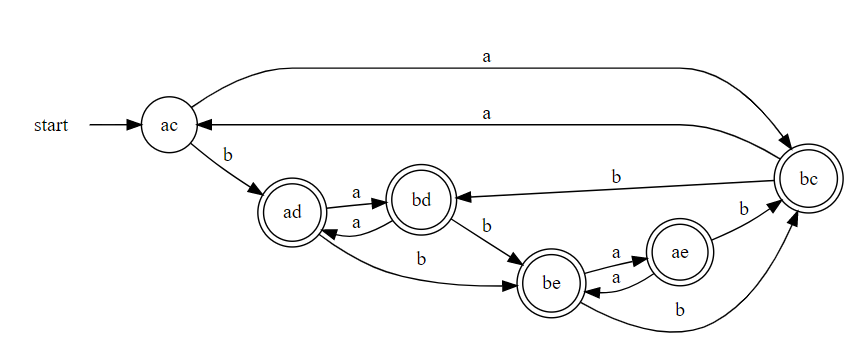
\includegraphics[0.5]{2.4.png}
    \item $L_{5} = L_{2} \textbackslash L_{3}$
\\ $L_{5} = L_{2} \textbackslash L_{3} = L_{2} \cap \overline L_{3}$
\\ Переименуем состояния чтобы было удобнее работать 
\\ $L_{2}$ :
\\ 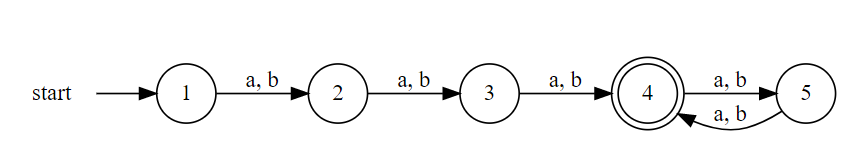
\includegraphics[0.5]{2.5.1(2).png}
\\ $\textbackslash L_{3}$:
\\ 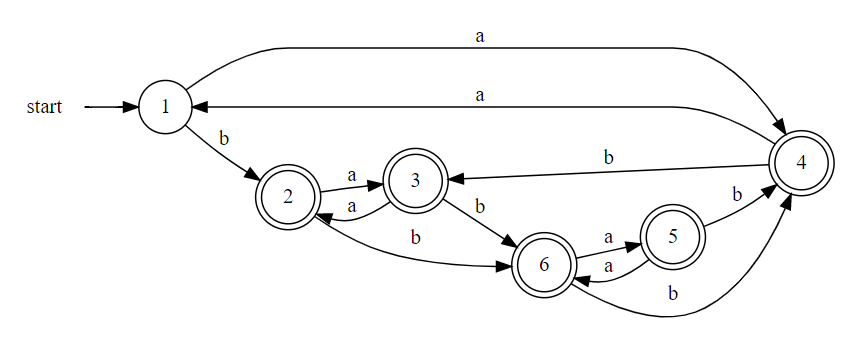
\includegraphics[0.5]{2.5.2(3).png}
\\ $\sum \begin{Bmatrix}
a, b
\end{Bmatrix}$
\\ $Q = \begin{Bmatrix}
11, 12, 13, 14, 15, 16, 21, 22, 23, 24, 25, 26, 31, 32, 33, 34, 35, 36, 41, \\42, 43, 44, 45, 46, 51, 52, 53, 54, 55, 56
\end{Bmatrix}$
\\ $s = <11>$
\\ $T = <42, 43, 44, 45, 46>$
\\ $L_{5} = L_{2} \textbackslash L_{3}$
\\ 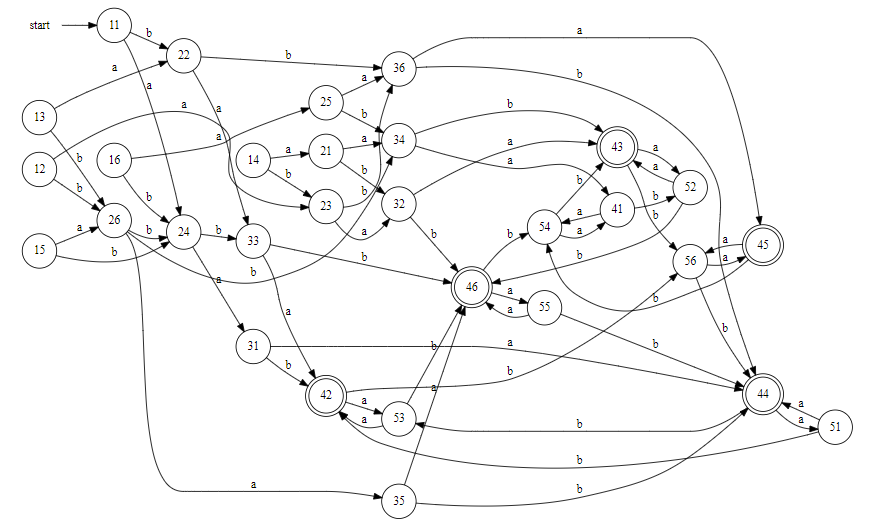
\includegraphics[0.5]{2.5pre.png}
\\ После упрощения 
\\ 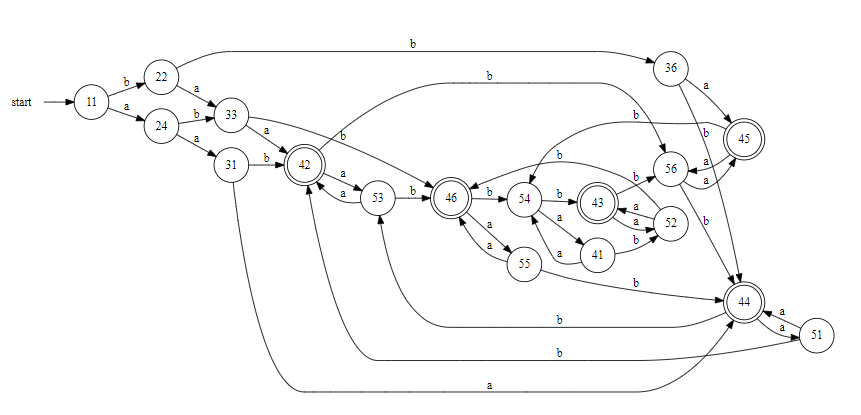
\includegraphics[0.5]{2.5post.png}
\end{enumerate}
\section{Задача 3}
\\ Построить минимальный ДКА, который допускает язык, описанный регулярным выражением
\begin{enumerate}
    \item (ab+aba)*a
\\ Построим в НДА:
\\ 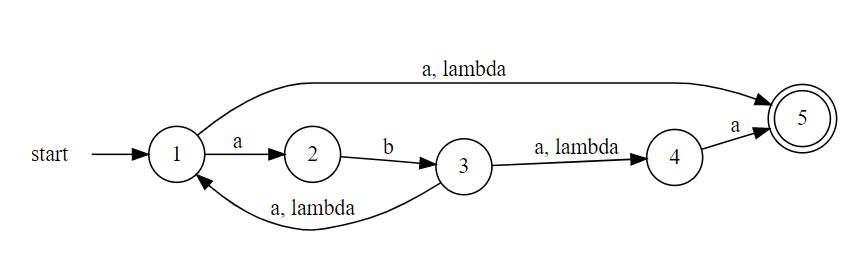
\includegraphics[0.5]{3.1pre.png}
\\ Построим эквивалентный ДКА по НКА по алгоритму Томпсона \\ 
\begin{tabular}{ | l | l | l | }
\hline
Q & a & b \\ \hline
1 & 25 & - \\ \hline
25 & - & 3 \\ \hline
3 & 1245 & - \\ \hline
1245 & 25 & 3 \\
\hline
\end{tabular}
\\ Минимальный ДКА:
\\ 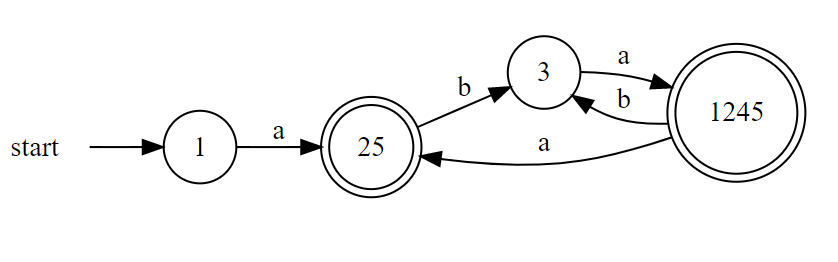
\includegraphics[0.5]{3.1post.png}
    \item a(a(ab)*b)*(ab)*
\\ Построим НKА:
\\ \includegraphics[0.5]{3.2.png}
\\ Нам повезло и это минимальный ДКА
    \item (a+(a+b)(a+b)b)*
\\ Построим НKА:
\\ \includegraphics[0.5]{3.3.1.png}
\\ Построим эквивалентный ДКА по НКА по алгоритму Томпсона \\ 
\begin{tabular}{ | l | l | l | }
\hline
Q & a & b \\ \hline
1 & 12 & 2 \\ \hline
12 & 123 & 23 \\ \hline
123 & 123 & 123 \\ \hline
23 & 3 & 13 \\ \hline
13 & 12 & 12  \\ \hline
2 & 3 & 3 \\ \hline
3 & - & 1 \\ 
\hline
\end{tabular}
\\ Построим ДКА
\\ \includegraphics[0.5]{3.3.2.png}
\\ Минимизируем: \\
\begin{tabular}{ | 1 | 1 | 1 | 1 | 1 | 1 | 1 | 1 | }
\hline
 & 1 & 2 & 3 & 12 & 13 & 23 & 123 \\ \hline
1 & & + & + & + & + & + & + \\ \hline
2 & + & & + & + & + & + & + \\ \hline
3 & + & + & & + & + & + & + \\ \hline
12 & + & + & + & & + & + & + \\ \hline
13 & + & + & + & + & & + & + \\ \hline
23 & + & + & + & + & + & & + \\ \hline
123 & +  & + & + & + & + & + &  \\
\hline
\end{tabular}
\\ Полученный ДКА минимальный
    \item (b+c)((ab)*c+(ba)*)*
\\ Построим НДА:
\\ \includegraphics[0.5]{3.4pre.png}
\\ Получен ДКА, минимизируем \\ 
\begin{tabular}{ | 1 | 1 | 1 | 1 | 1 | 1 | 1 | 1 | 1 | 1 | }
\hline
 & 1 & 2 & 3 & 4 & 5 & 6 & 7 & 8 & 9\\ \hline
1 & & + & + & + & + & + & + & + & + \\ \hline
2 & + & & + & + & + & + & + & + & + \\ \hline
3 & + & + & & + & + & + & + & + & + \\ \hline
4 & + & + & + & & + & + & + & + & + \\ \hline
5 & + & + & + & + & & + & + & + &  \\ \hline
6 & + & + & + & + & + &  & + & + & + \\ \hline
7 & + & + & + & + & + & + &  & + & + \\ \hline
8 & + & + & + & + & + & + & + &  & + \\ \hline
9 & + & + & + & + &  & + & + & + &  \\
\hline
\end{tabular}
\\
\\ Перестроим с состояниями $<1, 2, 3, 4, 59, 6, 7, 8>$
\\ \includegraphics[0.5]{3.4post.png}
    \item $(a+b)^{+}(aa+bb+abab+baba)(a+b)^{+}$
\\ Построим НKА:
\\ \includegraphics[0.5]{3.5pre.png}
\\ ДКА : \\
\begin{tabular}{ | l | l | l | }
\hline
Q & a & b \\ \hline
1 & 2 & 2 \\ \hline
2 & 23 & 24 \\ \hline
23 & 239 & 245 \\ \hline
239 & 23910 & 24510 \\ \hline
245 & 2368 & 249 \\ \hline
24 & 236 & 249 \\ \hline
23910 & 23910 & 24510 \\ \hline
24510 & 236810 & 24910 \\ \hline
2368 & 239 & 24579 \\ \hline
249 & 23610 & 24910 \\ \hline
236 & 239 & 2457 \\ \hline
236810 & 23910 & 2457910 \\ \hline
24910 & 23610 & 24910 \\ \hline
24579 & 2368910 & 24910 \\ \hline
23610 & 23910 & 245710 \\ \hline
2457 & 23689 & 249 \\ \hline
2457910 & 2368910 & 24910 \\ \hline
2368910 & 23910 & 2457910 \\ \hline
245710 & 2368910 & 24910 \\ \hline
23689 & 23910 & 2457910 \\ 
\hline
\end{tabular}
\\ \includegraphics[0.5]{3.5post.png}
\end{enumerate}
\section{Задача 4}
\\ Построить автомат если язык регулярный или доказать обратное с помощью леммы о разростании 
\begin{enumerate}
    \item $L = \begin{Bmatrix}
(aab)^{n}b(aba)^{m} | n\geq 0, m \geq 0
\end{Bmatrix}$
\\ Можнос построить 
\\ \includegraphics[0.5]{4.1.png}
    \item $L = \begin{Bmatrix}
uaav | u \in \begin{Bmatrix}
a, b
\end{Bmatrix}^{*},v \in \begin{Bmatrix}
a, b
\end{Bmatrix}^{*}, |u|_{b} \geq |v|_{a}
\end{Bmatrix}$
\\ Фиксируем n 
\\ Рассмотрим частный случай 
    \item $L = \begin{Bmatrix}
a^{m}w | w \in \begin{Bmatrix}
a, b
\end{Bmatrix}^{*}, 1 \leq |w|_{b} \leq m
\end{Bmatrix}$
    \item $L = \begin{Bmatrix}
a^{k}b^{m}a^{n} | k = n \vee m > 0
\end{Bmatrix}$
    \item $L = \begin{Bmatrix}
ucv | u \in \begin{Bmatrix}
a, b
\end{Bmatrix}^{*}, v \in \begin{Bmatrix}
a, b
\end{Bmatrix}^{*}, u \neq v^{R}
\end{Bmatrix}$
\end{enumerate}
\end{document}